%%%%%%%%%%%%
%%
%%%%%%%%%%%%

\section{Background}

\subsection{Core PROV model} \label{sec:prov-core}

We now introduce the core elements of the PROV model, which forms the basis for the grouping operator.
%
We maintain a dual view of provenance, both as a relational model (with binary relations) and as a graph model. Viewed as a relational model, PROV includes three types of elements: Entities ($\en$), Activities ($\act$), and Agents ($\ag$), and several types of relations amongst them. 
In line with the description in~\citep{w3c-prov-dm} (sec. 2), PROV is defined by the following core relations, with common abbreviations in brackets. 

\begin{eqnarray*}
Used~~(\used)  & \subseteq & \act \times \en \\
WasGeneratedBy~~(\wgby) & \subseteq  & \en \times \act \\
WasDerivedFrom~~(\wdf) & \subseteq   & \en \times \en \\
WasInvalidatedBy~~(\inv) &  \subseteq &  \en \times \act \\
WasAssociatedWith~~(\waw) & \subseteq & \act \times \ag \\
ActedOnBehalfOg~~(\delegate) & \subseteq & \ag \times \ag \\ 
WasAttributedTo~~(\attrTo) & \subseteq & \en \times \ag \\
WasInformedBy~~(\wasInfBy) & \subseteq & \act \times \act
\end{eqnarray*}


\begin{figure}
\centering
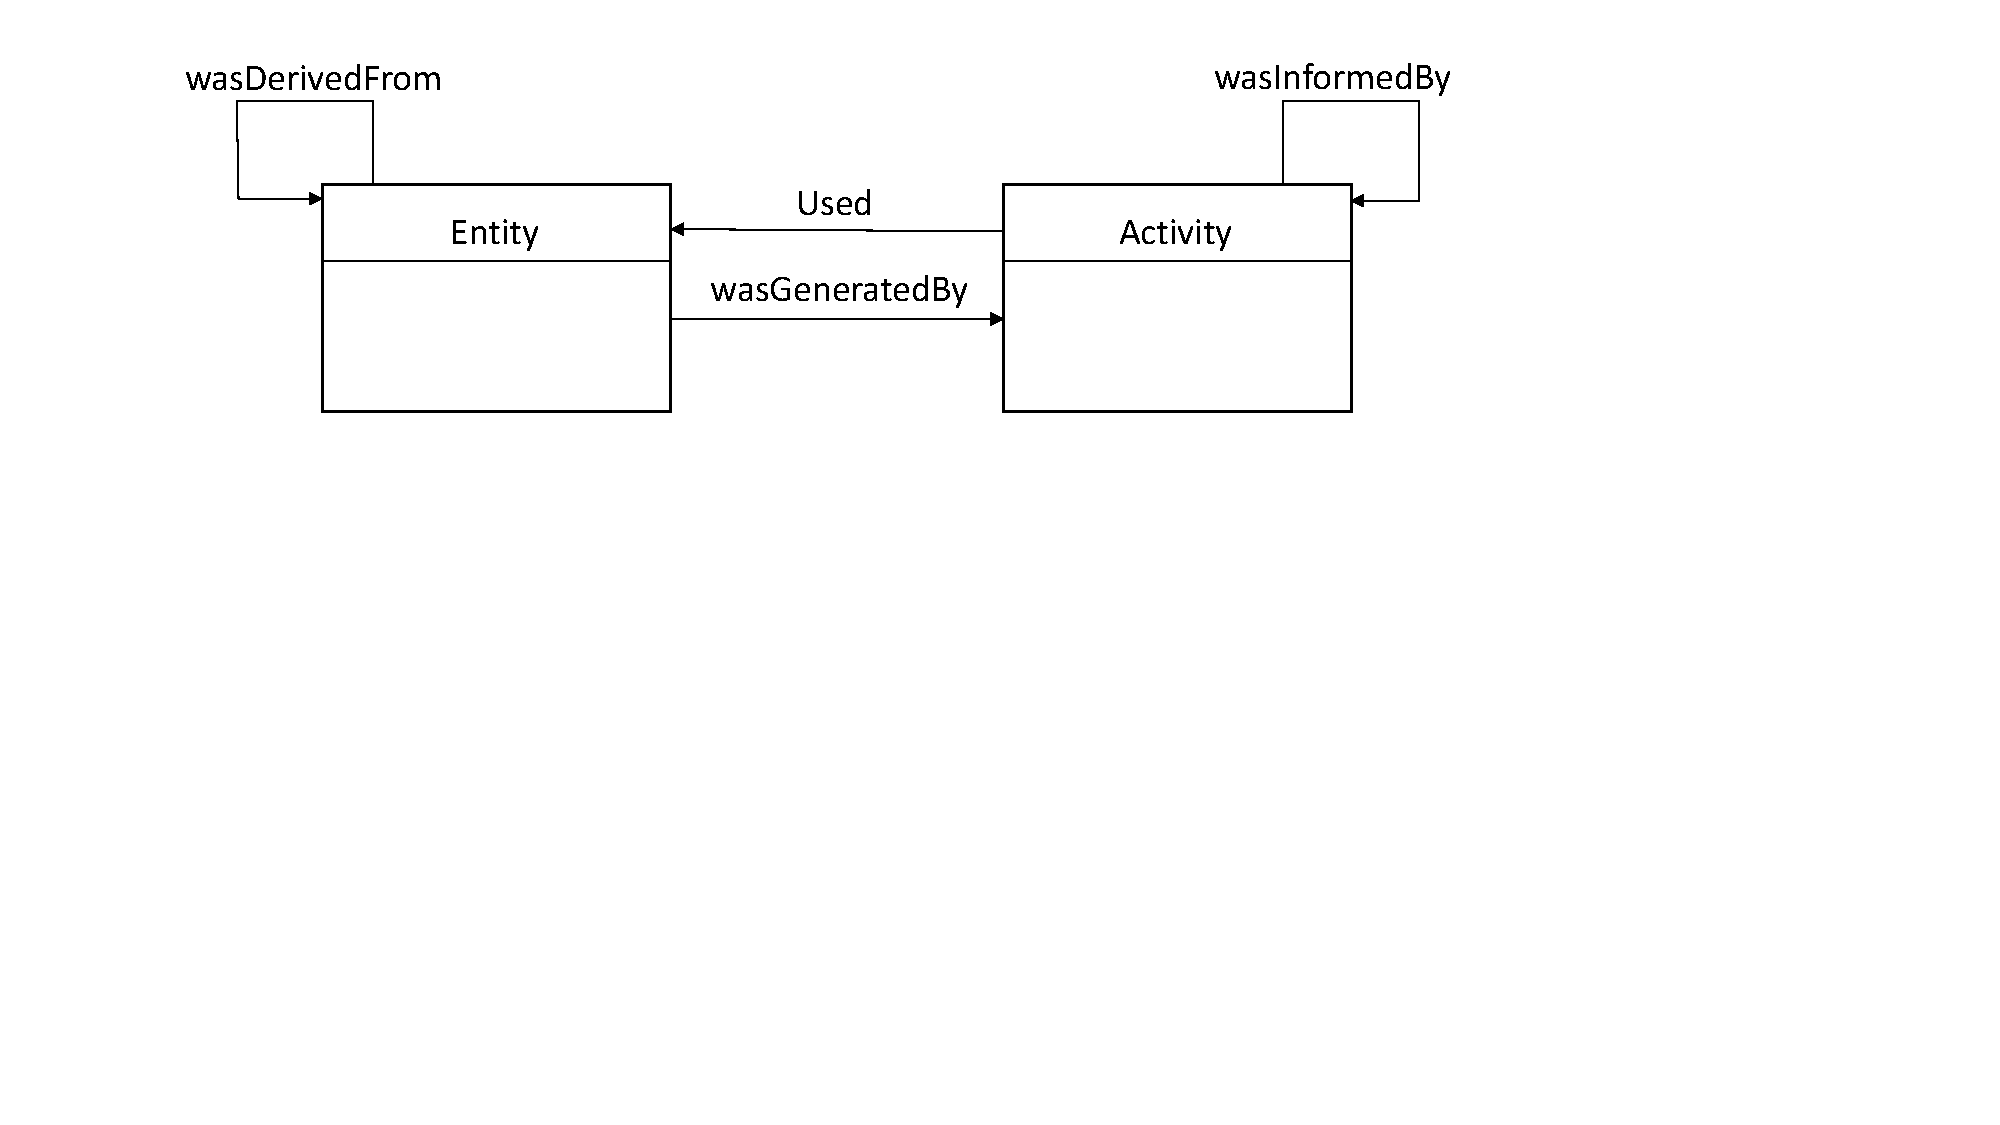
\includegraphics[scale=.45]{figures/prov-essentials.pdf} 
\caption{Core elements of the PROV model, adapted from~\citep{w3c-prov-dm}}
\label{fig:prov-core}
\end{figure}

%\subsection{Bipartite PROV: $\guEA$}  \label{sec:prov-guea}
These are summarized in Fig.~\ref{fig:prov-core}.
%
Initially, we are going to restrict ourselves to an even simpler model, consisting only of $\en$, $\act$, and relations $\used$ and $\wgby$. Agents and the relations that involve them are introduced in Sec.~\ref{sec:agents-abstraction}.
%
Further extensions to the additional relations --- $\wdf$ and $\wasInfBy$ --- are straightforward and are not considered in detail.

%
An instance  of the model is a provenance document $D$, consisting of sets $en \in \en$ and $act \in \act$ of symbols, and sets of relation instances $\{ \wgby(e,a)  | e \in \en, a \in \act \} \cup   \{ \used(a,e)  | e \in \en, a \in \act\}$. 

%
As these relations are binary, we view $D$ as a digraph $G=(V,E)$, where $V= \en \cup \act$, and each relation instance maps to a labelled directed edge. By convention, we orient these edges from right to left, to denote that the relation ``points back to the past''. Thus:
$a \xleftarrow{\wgby} e \in E$ iff $\wgby(e,a) \in D$, and $e \xleftarrow{\used} a \in E$ iff $\used(a,e) \in D$.
%
We denote the label associated to edge $(v_i, v_j)$ as $\elabel(v_i,v_j)$. 

%
Note that, by definition of the relations, $G$ is a bipartite graph.
We denote the set of all such graphs by $\guEA$, to indicate that they only contain $\en$ and $\act$ nodes, and $\wgby$ and $\used$ edges. In Sec.~\ref{sec:agents-abstraction} we are going to extend this set to include agents as well as additional relations.
Fig.~\ref{fig:baseline-ug-ae} portrays a simple $\guEA$ graph that we will be using as a running example.

\begin{figure}
\centering
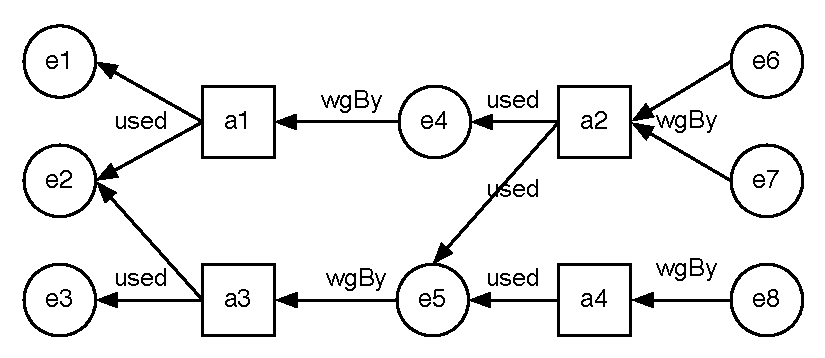
\includegraphics[scale=.6]{figures/baseline-ug-ae.pdf} 
\caption{$\guEA$ provenance graph used as a running example to illustrate abstraction by grouping}  \label{fig:baseline-ug-ae}
\end{figure}

\subsection{Events in $\guEA$}

\label{sec:events}

Central to PROV is the notion that provenance is marked by events. A partial order is defined over events, so that it may or may not be possible to establish whether or not one event precedes another. 
%
Events occur instantaneously, and they mark the lifetime boundaries of Entities (generation, invalidation), Activities (start, end), and Agents (start, end), as well as some of the interactions amongst those elements. These include the generation and usage of an entity by an activity, attribution of an entity to an agent, and more. More specifically, the PROV-CONSTRAINTS document~\citep{w3c-prov-constraints} defines the following types of events (quoted verbatim from Sec. 2.2):

\begin{itemize} %
	\item\textbf{An activity start event} is the instantaneous event that marks the instant an activity starts.
	
	\item\textbf{An activity end event} is the instantaneous event that marks the instant an activity ends.
	
	\item\textbf{An entity generation event} is the instantaneous event that marks the final instant of an entity's creation timespan, after which it is available for use. The entity did not exist before this event.
	
	\item\textbf{An entity usage event}  is the instantaneous event that marks the first instant of an entity's consumption timespan by an activity. The described usage had not started before this instant, although the activity could potentially have used the same entity at a different time.
	
	\item\textbf{An entity invalidation event} is the instantaneous event that marks the initial instant of the destruction, invalidation, or cessation of an entity, after which the entity is no longer available for use. The entity no longer exists after this event.
	
\end{itemize}
%\end{description}

In order to formally express events, we introduce a set $\Ev$ of event symbols, with a pre-order\footnote{Recall that a pre-order is a binary relation with reflexivity and transitivity, but no symmetry or anti-symmetry.} $\preorder \subset \Ev \times \Ev$, and the following set of partial functions that associate events to elements and relations in a provenance instance:
\begin{align*}
start: \act \rightarrow \Ev \\
end: \act \rightarrow \Ev \\
ev: \wgby \cup \used \cup \inv \rightarrow \Ev
\end{align*}	
As an example, in the graph of Fig.~\ref{fig:baseline-ug-ae} the generation relation $\wgby(e_4, a_1)$ has an associated generation event $ev(\wgby(e_4, a_1))$, whilst $a_1$ has start and / or end events, written $start(a_1)$ and $end(a_1)$, respectively. Similarly, usage of $e_4$ by $a_2$ is marked by event $ev(\used(a_2, e_4))$. Finally, if $e_4$ had been invalidated by some $a$ (not in the figure), this would be represented by an invalidation event $ev(\inv(e_4,a))$.

Temporal constraints involving events, and expressed by means of their pre-order relation $\preorder$, play a key role in the definition of \textit{valid} provenance instances, as described next.

\subsection{Constraints and valid $\guEA$ graphs}
\label{sec:prov-constraints}

As mentioned earlier, our goal in this work is to define transformations of a valid PROV instance into new valid instance, whilst providing obfuscation by abstracting out some of its details. Validity is defined in terms of a set of constraints, as stated in the PROV-CONSTRAINTS document~\citep{w3c-prov-constraints}.
%
For instance, Constraint 55 states that the Entities and Activities are disjoint:  $\en \cap \act = \emptyset$.
Thus, a document $D$ that contains both statements (1) $a_1 \used~e_1$ and (2) $e_1 \used ~a_1$ cannot be valid, because by definition of $\used$ given earlier, (1) entails 
$e_1 \in \en$, $a_1 \in \act$, while (2) entails $a_1 \in \en$, $e_1 \in \act$, violating the constraint.

Note that disjointness constraint 55 entails that $\guEA$ graphs are bipartite.

In this paper we are mainly concerned with temporal constraints, which apply to $\guEA$ instances and determine the admissible partial ordering of the event types introduced in the previous section.
With reference to a graph $\pg$, these are (including constraint (55) above, and using the original numbering in~\citep{w3c-prov-constraints})

\begin{itemize}
	
	\item\textbf{C1: entity-activity-disjoint (Constraint 55):} \[\en \cap \act = \emptyset\]
	
	\item\textbf{C2: generation-generation-ordering (Constraint 39):}  If an entity is generated by more than one activity, then the generation events must all be simultaneous.
	
	Let 
	$gen_1 = ev(\wgby(e, a_1))$, $gen_2 = ev(\wgby(e, a_2)) \in \pg$. Then  \[gen_1  \preorder  gen_2, \quad gen_2 \preorder gen_1\] must hold.
	
	\item\textbf{C3: generation-precedes-usage(Constraint 37):} A generation event for an entity must precede any usage event for that entity.
	%
	For any $a \in \act$ such that $\used(a,e) \in \pg$, \[	ev(\wgby(e, a)) \preorder ev(\used(a,e))\] must hold.
	
	\item\textbf{C4: generation-precedes-invalidation (Constraint 36):} The generation event (or, more accurately, the set of simultaneous generation events) for an entity must precede the invalidation event.
	
	For any $a,a' \in \act$ such that $\wgby(e, a))$, $\inv(e,a') \in \pg$ :
	\[ ev(\wgby(e, a)) \preorder ev(\inv(e,a')) \]
	
	\item\textbf{C5: usage-precedes-invalidation (Constraint 38):} Any usage event for an entity must precede the invalidation event.
%	
	For any $a,a' \in \act$ such that $\used(a,e))$, $\inv(e,a') \in \pg$ :
	\[ ev(\used(a,e)) \preorder ev(\inv(e,a')) \]
	
	\item\textbf{C6: usage-within-activity (Constraint 33):} Any usage of $e$ by $a$ cannot precede the start of $a$ and must precede the end of $a$. For any $e\in \en, a \in \act$ such that $\used(a,e) \in \pg$:
	\[start(a) \preorder ev(\used(a,e))   \preorder end(a)\]
	
	\item\textbf{C7: generation-within-activity (Constraint 34):} The generation of $e$ by $a$ cannot precede the start of $a$ and must precede the end of $a$.
	Let $\wgby(e,a) \in \pg$:
	\[ start(a) \preorder ev(\wgby(e,a))  \preorder ev(a)\]
	
	\item\textbf{C8: invalidation-invalidation-ordering (Constraint 40):}	If an entity is invalidated by more than one activity, the events must all be simultaneous.
	\begin{align*}
		&\text{if } \inv(e,a_1), \inv(e,a_2) \in \pg \\
		&\text{ then } ev(\inv(e,a_1)) = ev(\inv(e,a_2)) 
	\end{align*}


\end{itemize}

Additional relevant constraints state that multiple start (resp. end, invalidation) events must all be simultaneous, and that the start event of an activity must precede the end event for that activity.
\\

\begin{definition}[Validity]
 A graph $G \in \guEA$ is valid iff it satisfies constraints C1-C8.
	\label{def:valid-guea}
\end{definition}

\comment{should finish off with a sign-post para here}
